\pdfminorversion=4 % for acroread
\documentclass[t]{beamer}
%\documentclass[t,handout]{beamer}

\usepackage[english]{babel}
\usepackage[utf8]{inputenc}
\usepackage{graphicx}
\usepackage{booktabs}

\usepackage{amsmath,amssymb}
\usepackage{listings}
\lstset{frame=lines,framesep=3pt,numbers=left,numberblanklines=false,basicstyle=\ttfamily\small}

\usepackage{subfig}
\usepackage{multicol}
\usepackage{appendixnumberbeamer}

\usepackage{tikz}
\usetikzlibrary{trees} 
\usetikzlibrary{shapes.geometric}
\usetikzlibrary{positioning,shapes,shadows,arrows,calc,mindmap}
\pgfdeclarelayer{background}
\pgfdeclarelayer{foreground}
\pgfsetlayers{background,main,foreground}
\tikzstyle{activity}=[rectangle, draw=white, rounded corners, text centered, text width=8em]
\tikzstyle{data}=[rectangle, draw=white, text centered, text width=8em]
\tikzstyle{myarrow}=[->, thick, draw=white]

% Define the layers to draw the diagram
\pgfdeclarelayer{background}
\pgfdeclarelayer{foreground}
\pgfsetlayers{background,main,foreground}


\usepackage{listings}
\lstset{numbers=left,
  showstringspaces=false,
  frame={tb},
  captionpos=b,
  lineskip=0pt,
  basicstyle=\ttfamily,
  extendedchars=true,
  stepnumber=1,
  numberstyle=\small,
  xleftmargin=1em,
  breaklines
}

 

\usetheme{Madrid}
\useinnertheme{rectangles}
\usecolortheme{whale}
\setbeamercolor{alerted text}{fg=blue}
\useoutertheme{infolines}
\setbeamertemplate{navigation symbols}{\vspace{-5pt}} % to lower the logo
\setbeamercovered{invisible}

\makeatletter
\setbeamertemplate{footline}
{
  \leavevmode%
  \hbox{%
  \begin{beamercolorbox}[wd=.333333\paperwidth,ht=2.25ex,dp=1ex,center]{author in head/foot}%
    \usebeamerfont{author in head/foot}\insertshortauthor
  \end{beamercolorbox}%
  \begin{beamercolorbox}[wd=.333333\paperwidth,ht=2.25ex,dp=1ex,center]{title in head/foot}%
    \usebeamerfont{title in head/foot}\insertshorttitle
  \end{beamercolorbox}%
  \begin{beamercolorbox}[wd=.333333\paperwidth,ht=2.25ex,dp=1ex,right]{date in head/foot}%
    \usebeamerfont{date in head/foot}\insertshortdate{}\hspace*{2em}
    \insertframenumber\hspace*{2ex} 
  \end{beamercolorbox}}%
  \vskip0pt%
}
\makeatother

\newcommand{\lit}[1]{{\footnotesize\color{black!70}[#1]}}
\newcommand{\litw}[1]{{\footnotesize\color{black!20}[#1]}}

\pgfdeclareimage[height=1.2cm]{coseallogo}{images/logos/coseal}
\pgfdeclareimage[height=1.2cm]{mlaad}{images/logos/ml4aad.png}
\pgfdeclareimage[height=1.2cm]{freiburg}{images/logos/freiburg}

\logo{\pgfuseimage{freiburg}}

\title[MLOAD]{Machine Learning and Optimization\\ for Algorithm Design}
\subtitle{ML Mini Competition}
\author{Marius Lindauer}
\institute{University of Freiburg}
\date{}
%\date{LION 2015, Lille, France}

% \AtBeginSection[] % Do nothing for \section*
% {
%   \begin{frame}{Outline}
%     \bigskip
%     \vfill
%     \tableofcontents[currentsection]
%   \end{frame}
% }


\begin{document}

% ----------------------------------------------------------------------
{
\setbeamertemplate{footline}{} % remove footer on first slide
	\frame[c]{
	\titlepage
	\begin{center}
	\vspace{-1.5cm}
	%
\includegraphics[height=5em]{images/logos/freiburg}\quad\quad
	%
\includegraphics[height=5em]{logo/coseal}\quad
	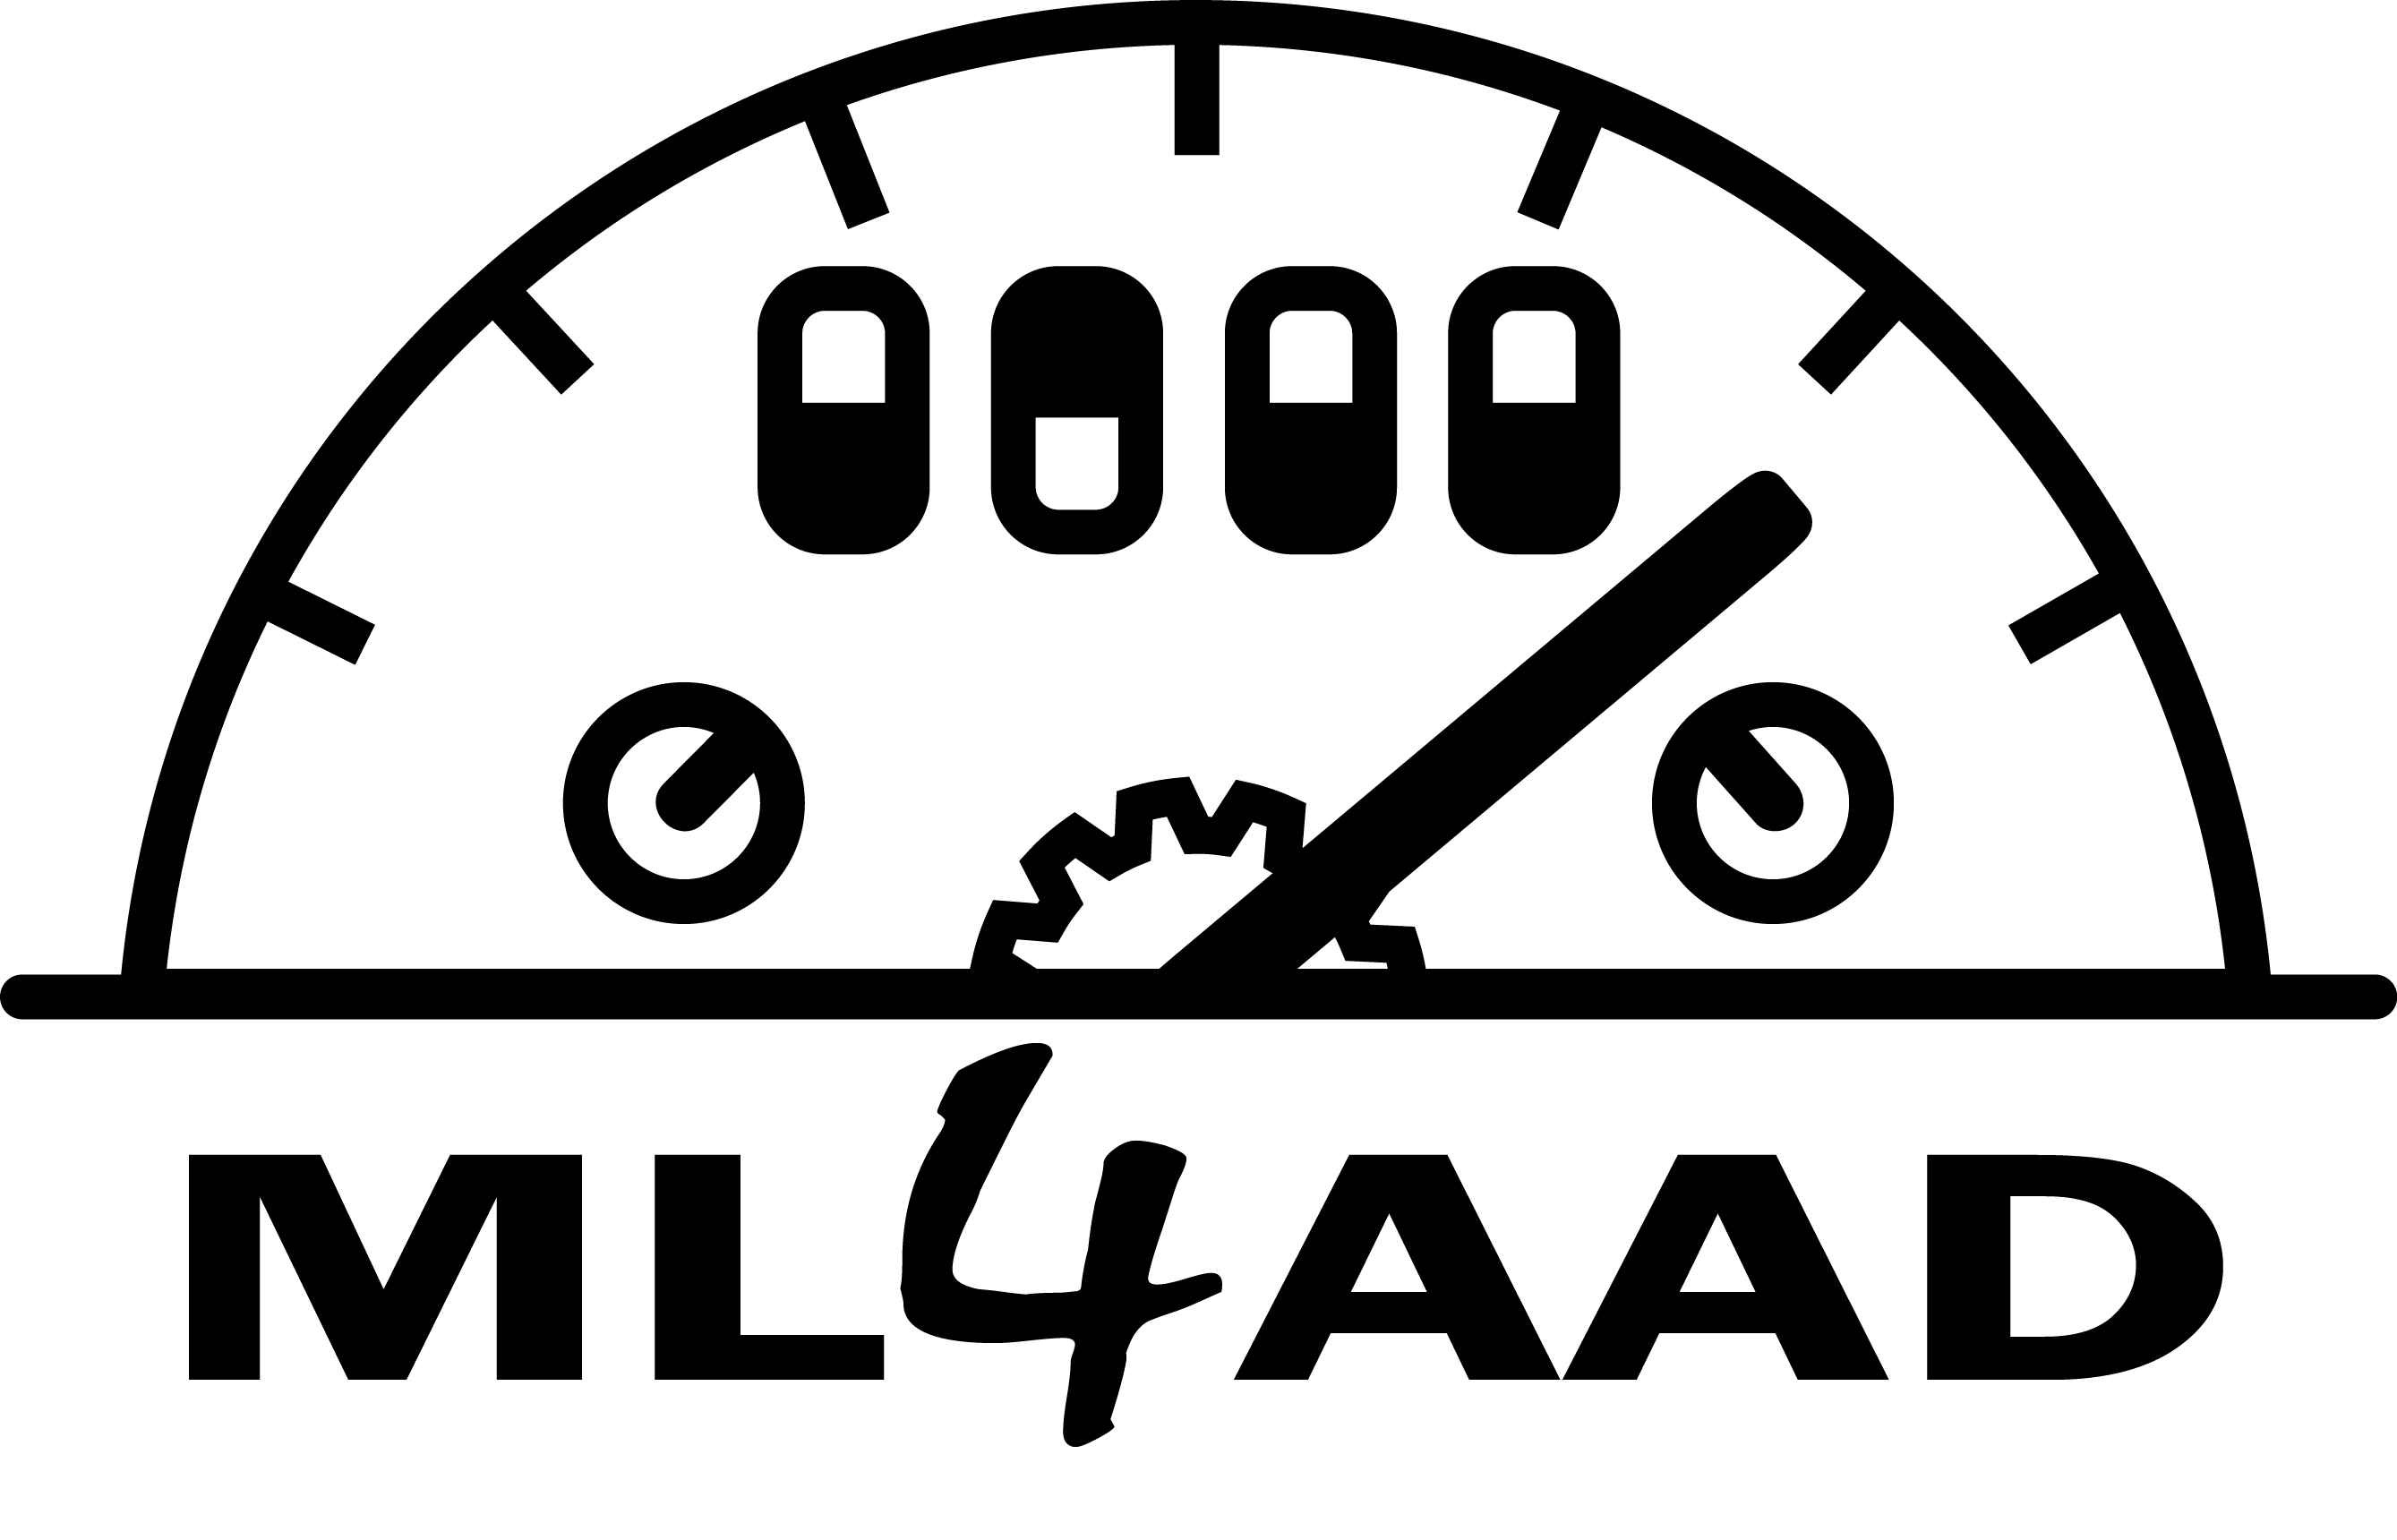
\includegraphics[height=5em]{images/logos/ml4aad.png}
	\end{center}
	}
}
\author{Lindauer}
\institute{}
%\logo{\pgfuseimage{mlaad}}
\logo{}

%----------------------------------------------------------------------------------
%----------------------------------------------------------------------------------
\begin{frame}[c, fragile]{Data Sets}

\small
\centering
\begin{tabular}{l | r | rrrr | rr}
\toprule
Set & \#D & \#F & \#Inform. & \#Redun. & \#Repeat. & \#Classes & \#Clusters\\
\midrule
Set1 & 1000 & 6 & 6 & 0 & 0 & 2 & 3\\
Set2 & 2000 & 10 & 6 & 4 & 0 & 2 & 2 \\
Set3 & 4000 & 10 & 2 & 6 & 2 & 2 & 2 \\
Set4 & 6000 & 12 & 12 & 0 & 0 & 2 & 4\\
Set5 & 1000 & 100 & 10 & 90 & 0 & 2 & 4\\
\bottomrule
\end{tabular}

\end{frame}
%----------------------------------------------------------------------------------
%----------------------------------------------------------------------------------
\begin{frame}[c, fragile]{Set 1}

\centering
\begin{tabular}{llr}
\toprule
Rank & Team & Accuracy\\
\midrule
\onslide<10->{1 & Ali Syed & 0.9495}\\
\onslide<9->{1 & Dzerin and Ernestus & 0.9495}\\
\onslide<8->{1 & Freidank and Negassi & 0.9495}\\
\onslide<7->{4 & Marben & 0.9394}\\
\onslide<6->{4 & Paiva & 0.9394}\\
\onslide<5->{4 & baseline & 0.9394}\\
\onslide<4->{7 & (Koller and Maas) & 0.9293}\\
\onslide<3->{8 & Rabald & 0.9192}\\
\onslide<2->{8 & Biedenkapp and Wunsch & 0.9192}\\
\onslide<1->{10 & (Aashiq and Ur-Rehman) & 0.8990}\\
\bottomrule
\end{tabular}

\end{frame}
%----------------------------------------------------------------------------------
%----------------------------------------------------------------------------------
\begin{frame}[c]{Set 2}

\centering
\begin{tabular}{llr}
\toprule
Rank & Team & Accuracy\\
\midrule
\onslide<10->{1 & Freidank and Negassi & 0.9799}\\
\onslide<9->{2 & Marben & 0.9749}\\
\onslide<8->{2 & (Koller and Maas) & 0.9749}\\
\onslide<7->{2 & Ali Syed & 0.9749}\\
\onslide<6->{2 & Dzerin and Ernestus & 0.9749}\\
\onslide<5->{6 & Rabald & 0.9698}\\
\onslide<4->{6 & Paiva & 0.9698}\\
\onslide<3->{6 & Biedenkapp and Wunsch & 0.9698}\\
\onslide<2->{9 & (Aashiq and Ur-Rehman) & 0.9397}\\
\onslide<1->{9 & baseline & 0.9397}\\
\bottomrule
\end{tabular}

\end{frame}
%----------------------------------------------------------------------------------
%----------------------------------------------------------------------------------
\begin{frame}[c]{Set 3}

\centering
\begin{tabular}{llr}
\toprule
Rank & Team & Accuracy\\
\midrule
\onslide<10->{1 & Freidank and Negassi & 0.8321}\\
\onslide<9->{2 & Rabald & 0.8246}\\
\onslide<8->{3 & Marben & 0.8221}\\
\onslide<7->{3 & Ali Syed & 0.8221}\\
\onslide<6->{5 & Dzerin and Ernestus & 0.8195}\\
\onslide<5->{6 & Biedenkapp and Wunsch & 0.8170}\\
\onslide<4->{7 & (Aashiq and Ur-Rehman) & 0.8145}\\
\onslide<3->{8 & (Koller and Maas) & 0.8120}\\
\onslide<2->{8 & Paiva & 0.8120}\\
\onslide<1->{10 & baseline & 0.8070}\\
\bottomrule
\end{tabular}

\end{frame}
%----------------------------------------------------------------------------------
%----------------------------------------------------------------------------------
\begin{frame}[c]{Set 4}

\centering
\begin{tabular}{llr}
\toprule
Rank & Team & Accuracy\\
\midrule
\onslide<10->{1 & Dzerin and Ernestus & 0.9182}\\
\onslide<9->{2 & Ali Syed & 0.9065}\\
\onslide<8->{3 & Biedenkapp and Wunsch & 0.9048}\\
\onslide<7->{4 & Marben & 0.8948}\\
\onslide<6->{5 & Paiva & 0.8915}\\
\onslide<5->{6 & Freidank and Negassi & 0.8848}\\
\onslide<4->{7 & Rabald & 0.8831}\\
\onslide<3->{8 & (Koller and Maas) & 0.8447}\\
\onslide<2->{9 & (Aashiq and Ur-Rehman) & 0.8164}\\
\onslide<1->{10 & baseline & 0.7997}\\
\bottomrule
\end{tabular}

\end{frame}
%----------------------------------------------------------------------------------
%----------------------------------------------------------------------------------
\begin{frame}[c]{Set 5}

\centering
\begin{tabular}{llr}
\toprule
Rank & Team & Accuracy\\
\midrule
\onslide<10->{1 & Dzerin and Ernestus & 0.9192}\\
\onslide<9->{2 & (Aashiq and Ur-Rehman) & 0.9091}\\
\onslide<8->{2 & Freidank and Negassi & 0.9091}\\
\onslide<7->{2 & Paiva & 0.9091}\\
\onslide<6->{2 & baseline & 0.9091}\\
\onslide<5->{6 & Rabald & 0.8990}\\
\onslide<4->{6 & Biedenkapp and Wunsch & 0.8990}\\
\onslide<3->{8 & Marben & 0.8889}\\
\onslide<2->{8 & (Koller and Maas) & 0.8889}\\
\onslide<1->{10 & Ali Syed & 0.5152}\\
\bottomrule
\end{tabular}

\end{frame}
%----------------------------------------------------------------------------------
%----------------------------------------------------------------------------------
\begin{frame}[c]{Final Results}

\centering
\begin{tabular}{llr}
\toprule
Rank & Team & Average Rank\\
\midrule
\onslide<10->{1 & Dzerin and Ernestus & 2.0000}\\
\onslide<9->{2 & Freidank and Negassi & 2.2000}\\
\onslide<8->{3 & Ali Syed & 3.6000}\\
\onslide<7->{4 & Marben & 4.2000}\\
\onslide<6->{5 & Paiva & 5.0000}\\
\onslide<5->{6 & Biedenkapp and Wunsch & 5.8000}\\
\onslide<4->{6 & Rabald & 5.8000}\\
\onslide<3->{8 & (Koller and Maas) & 6.6000}\\
\onslide<2->{9 & baseline & 7.0000}\\
\onslide<1->{10 & (Aashiq and Ur-Rehman) & 7.4000}\\
\bottomrule
\end{tabular}


\end{frame}
%----------------------------------------------------------------------------------
%----------------------------------------------------------------------------------
\begin{frame}[c]{Place 3: Ali Syed}

\begin{itemize}
  \item SVM
  \item gamma $0.69$ and RBF kernel (found by random sampling)
  \item preprocessing: StandardScaler
\end{itemize}


\end{frame}
%----------------------------------------------------------------------------------
%----------------------------------------------------------------------------------
\begin{frame}[c]{Place 2: Freidank and Negassi}

\begin{itemize}
  \item \texttt{auto-sklearn} 
  \item optimized parameters of \texttt{auto-sklearn} with SMAC
\end{itemize}

\end{frame}
%----------------------------------------------------------------------------------
%----------------------------------------------------------------------------------
\begin{frame}[c]{Place 1: Dzerin and Ernestus}

\begin{itemize}
  \item SVM with a grid search on 3-fold CV to tune the parameters
  \begin{itemize}
  	\item standard scaler or no pre-processing
  	\item kernel: RBF or polynomial
  	\item penalty: 0.7, 1.0, 1.3 or 1.6
  \end{itemize}
\end{itemize}


\end{frame}
%----------------------------------------------------------------------------------
%----------------------------------------------------------------------------------
\end{document}
